\chapter{Układ sterowania i instrumentacji}
\label{cha:ch3_uklad_ster_i_instrumentacji}

Do odczytywania danych z obiektu i sterowania nim wykorzystano opisany w tym rozdziale układ sterowania i instrumentacji (\cref{fig:schemat_ukl_sterowania_instrumentacji}). W jego sercu znajduje się przemysłowy sterownik PLC, który odczytuje dane o położeniu kulki z dwóch czujników odległości oraz położenie kątowe wału silnika z~enkodera. Dodatkowo do sterownika podłączony został czujnik bazowania oraz przyciski: \texttt{START} (NO), \texttt{STOP} (NC). Na wyjścia sterownika podłączony został mostek H kontrolujący silnik oraz dioda sygnalizacyjna.

% TODO: zweryfikować podłączenie przycisków

\begin{figure}[H]
    \centering
    % TODO: przerobić rysunek w Inkscape
    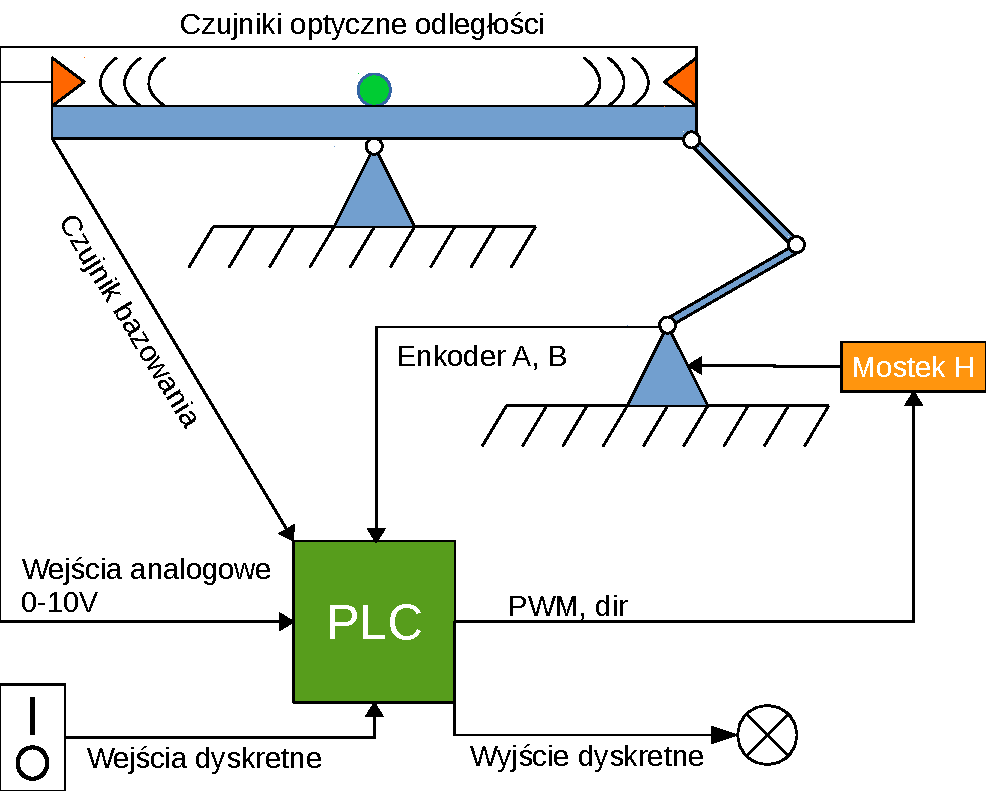
\includegraphics[width=0.7\textwidth]{schemat_ukladu3}
    \caption{Schemat układu sterowania i instrumentacji wraz z zaznaczonymi połączeniami.}
    \label{fig:schemat_ukl_sterowania_instrumentacji}
\end{figure}

%%%%%%%%
\section{Sterownik PLC}
\label{sec:ch3_PLC}

Wykorzystany w pracy sterownik PLC to Siemens S7-1211C DC/DC/DC. Działa on na napięciu stałym \SI{24}{V}, posiada 6 wejść dyskretnych \SI{24}{V}, 4 tranzystorowe wyjścia dyskretne \SI{24}{V} i 2 napięciowe wejścia analogowe \SIrange[range-units=single]{0}{10}{V}.

W celu ułatwienia komunikacji między sterownikiem i elektroniką opartą o logikę \SI{5}{V} (więcej w podrozdziale \ref{sec:ch3_systemy_napiec}), został on rozszerzony o dodatkową płytkę sygnałową SB 1223 działającą na logice \SI{5}{V}; dodaje ona po 2 wejścia i~wyjścia dyskretne \SI{5}{V}.

Podstawowe parametry sterownika oraz płytki sygnałowej zostały zebrane w tabeli \ref{tab:parametry_PLC_SB}:

\begin{table}[H]
    \centering
    \begin{threeparttable}
        \caption{Podstawowe parametry sterownika PLC Siemens S7-1211C i płytki sygnałowej Siemens SB 1223\tnote{a}.}
        \label{tab:parametry_PLC_SB}
        
        \begin{tabularx}{\textwidth}{p{5cm} | p{5cm} | p{5cm} }
            \toprule
            Nazwa & Siemens S7-1211C & Siemens SB 1223 \\
            \midrule
            Napięcie zasilania & \SI{24}{V} DC & \SI{5}{V} DC \\
            \midrule
            Ilość wejść cyfrowych & 6 & 2 \\
            Ilość wyjść cyfrowych & 4 & 2 \\
            Ilość wejść analogowych & 2 & 0 \\
            Ilość wyjść analogowych & 0 & 0 \\
            Typ wejść cyfrowych & \textit{sink-source} & \textit{source} \\
            Typ wyjść cyfrowych & półprzewodnikowe MOSFET \textit{source} & półprzewodnikowe MOSFET \textit{sink-source} \\
            Typ wejść analogowych & Napięciowe \SIrange[range-units=single]{0}{10}{V} & n.d. \\
            \midrule
            Szybkie liczniki & Do 6 z częstotliwością \SI{100}{kHz}\tnote{b} & Do 2 z częstotliwością \SI{200}{kHz}\tnote{c} \\
            Wyjścia impulsowe & Do 4 z częstotliwością \SI{100}{kHz} & Do 2 z częstotliwością \SI{200}{kHz} \\
            \midrule
            Pamięć robocza & \SI{30}{kB} & n.d. \\
            Pamięć ładowania & \SI{1}{MB} & n.d. \\
            Pamięć trwała & \SI{10}{kB} & n.d. \\
            \midrule
            Czas wykonywania instrukcji boolowskich & \SI{0,08}{\micro\second}/instrukcję & n.d. \\
            Czas wykonywania operacji na typie WORD & \SI{1,7}{\micro\second}/instrukcję & n.d. \\
            Czas wykonywania operacji na typie REAL & \SI{2,3}{\micro\second}/instrukcję & n.d. \\
            \bottomrule
        \end{tabularx}
        
        \begin{tablenotes}
            \footnotesize
            \item[a] opracowanie własne na podstawie \cite{S7MANUAL},
            \item[b] w trybie kwadraturowym wykorzystywane są dwa wejścia, a~maksymalna częstotliwość wynosi \SI{80}{kHz},
            \item[c] w trybie kwadraturowym wykorzystywane są dwa wejścia, a~maksymalna częstotliwość wynosi \SI{160}{kHz}.
        \end{tablenotes}
    \end{threeparttable}
\end{table}

% TODO: dodaj zdjęcia

%%%%%%%%
\section{Silnik z reduktorem i enkoderem}
\label{sec:ch3_uklad_napedowy}

Jak już zasygnalizowano w rozdziale \ref{sec:ch2_przeniesienie_napedu}, w pracy użyto silnika prądu stałego (komutatorowy, z~magnesami trwałymi). Silnik sprzężony jest z~zębatą przekładnią redukcyjną o przełożeniu \num{18,75}:\num{1}. Za silnikiem umieszczony jest enkoder inkrementalny kwadraturowy o~64 impulsach na obrót wału, co daje 1200 impulsów za przekładnią.

Wybrany silnik stanowi dobry kompromis między złożonością, wydajnością i ceną. Dyskusja na temat możliwości zastosowania innych typów napędów została przeprowadzona w dodatku \ref{appA_warianty_zespolu_napedowego}.

Producent silnika nie dostarcza pełnej dokumentacji, a jedynie kilka wybranych parametrów. Wymusiło to analityczne lub eksperymentalne wyznaczenie pozostałych wymaganych do zamodelowania silnika parametrów. Wszystkie parametry zostały przedstawione w tabeli \ref{tab:parametry_silnika} poniżej.

\begin{table}[h]
    \centering
    \begin{threeparttable}
        \caption{Parametry fizyczne, elektryczne i mechaniczne silnika, enkodera i przekładni\tnote{a}.}
        \label{tab:parametry_silnika}
        
        \begin{tabularx}{0.6\textwidth}{l | l}
            \toprule
            Średnica & \SI{37}{\milli\meter} \\
            Długość & \SI{68}{\milli\meter} \\
            Masa & \SI{215}{g} \\
            Średnica wału & \SI{6}{\milli\meter} \\
            \midrule
            Przełożenie przekładni & \num{18,75}:\num{1} \\
            \midrule
            Napięcie znamionowe & \SI{12}{\volt} \\
            Prędkość znamionowa & \SI{52,36}{\radian\per\second} \\
            Prąd znamionowy & \SI{300}{\milli\ampere} \\
            Prąd zatrzymania silnika & \SI{5000}{\milli\ampere} \\
            Moment zatrzymania silnika & \SI{0,59}{\newton\meter} \\
            \midrule
            Rezystancja\tnote{b} & \SI{2,4}{\ohm} \\
            Stała SEM rotacji\tnote{b} $K_e$ & \SI{0,2154}{\volt\per\radian\per\second} \\
            Stała momentu\tnote{b} $K_t$ & \SI{0,2154}{\newton\meter\per\ampere} \\
            Współczynnik tarcia wiskotycznego\tnote{b} $\beta$ & \num{0,00161} \\
            Współczynnik tarcia suchego\tnote{b} $b$ & \num{0,019} \\
            Moment bezwładności przekładni i wału\tnote{c} $J$ & \num{0,00123} \\
            \bottomrule
        \end{tabularx}
        
        \begin{tablenotes}
            \footnotesize
            \item[a] opracowanie własne na podstawie \cite{SILNIK_MANUAL},
            % TODO: zaktualizuj odnośniki
            \item[b] zidentyfikowano analitycznie, więcej w rozdziale \ref{cha:ch6_identyfikacja},
            \item[b] zidentyfikowano eksperymentalnie, więcej w rozdziale \ref{cha:ch6_identyfikacja}.
        \end{tablenotes}
    \end{threeparttable}
\end{table}

Silnik sterowany jest przez PLC za pomocą układu mostka H. Został on dobrany tak, by spełniać wymagania elektryczne silnika w pracy znamionowej. Sterowany jest sygnałem PWM o częstotliwości przenoszenia \SI{20}{\kilo\hertz}. Dodatkowym sygnałem jest binarny sygnał kierunku obrotu silnika.

% TODO: sposób wyznaczania kąta pochylenia belki, mostek H - parametry

%%%%%%%%
\section{Czujniki odległości}
\label{sec:ch3_czujniki_odleglosci}

% TODO: opis czujników, charakterystyki, położenie, sposób wyznaczania pozycji

%%%%%%%%
\section{Czujnik bazowania}
\label{sec:ch3_czujnik_bazowania}

% TODO: transoptor szczelinowy, sposób montażu, schemat połączeń

%%%%%%%%
\section{Okablowanie i zabezpieczenia}
\label{sec:ch3_okablowanie_zabezpieczenia}

% TODO: zdjęcie "szafy"

%%%%%%%%
\section{Systemy napięć}
\label{sec:ch3_systemy_napiec}

% TODO: 5V, 12V, 24V

%%%%%%%%
\section{Podsumowanie}


%---------------------------------------------------------------------------